\section{Population Vs. Sample Distributions}
    We often assume the existence of a probability distribution for a given scenario.
    However the problem is we don't always know what this distribution is.
    One thing we can do to try and get a better understanding of it is to make measurements and look at the distribution of these measurements.
    The underlying probability distribution is called the population, or parent, distribution, and the distribution of the measurements is called the sample distribution.
    
    A simple example of this is tossing coins.
    Say we toss 4 coins, the population distribution tells us we should expect 2 heads.
    However this isn't guaranteed to happen every time.
    If we repeat this 4 coin toss 10 times we may get the following number of heads, \(X\):
    \[X = 4, 3, 2, 2, 2, 3, 1, 3, 1, 2.\]
    There is also a formula, 
    \[P_n(X) = \frac{n!}{X!(n - X)!}\left(\frac{1}{2}\right)^n,\]
    that gives the probability of getting \(X\) heads when you toss \(n\) coins.
    This is based on the binomial distribution which we will cover later.
    \begin{figure}[ht]
        \centering
        \begin{subfigure}{0.4\textwidth}
            \centering
            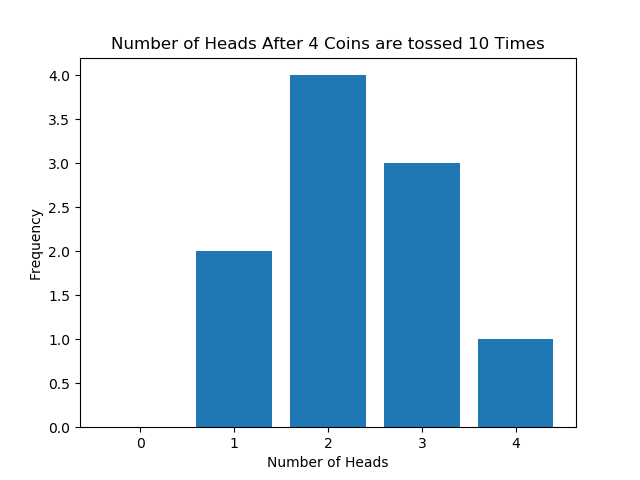
\includegraphics[scale=0.35]{coin_toss_results.png}
            \caption{Results of tossing 4 coins 10 times.}
            \label{fig:results of tossing 4 coins}
        \end{subfigure}
        \begin{subfigure}{0.4\textwidth}
            \centering
            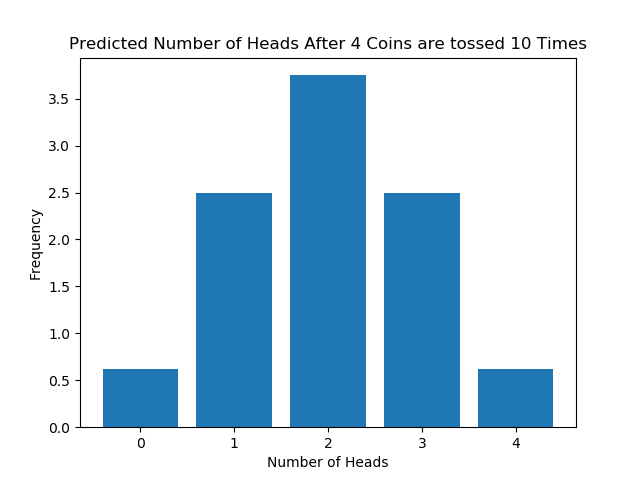
\includegraphics[scale=0.35]{coin_toss_prediction.png}
            \caption{Predicted number of heads for tossing 4 coins 10 times.}
            \label{fig:prediction of tossing 4 coins}
        \end{subfigure}
        \caption{Sample distribution vs. population distribution for counting the number of heads in four coin tosses.}
    \end{figure}
    The results of this experiment are plotted in figure~\ref{fig:results of tossing 4 coins} and the prediction is plotted in figure~\ref{fig:prediction of tossing 4 coins}.
    As you can see they are close but not quite the same.
    In general as we increase the number of times that we repeat an experiment we expect the results to look more and more like the prediction.
    We see this in figure~\ref{fig:10000 repeats} where the experiment was repeated 10000 times instead of 10 and the results and prediction are much closer.
    \begin{figure}[ht]
        \centering
        \begin{subfigure}{0.35\textwidth}
            \centering
            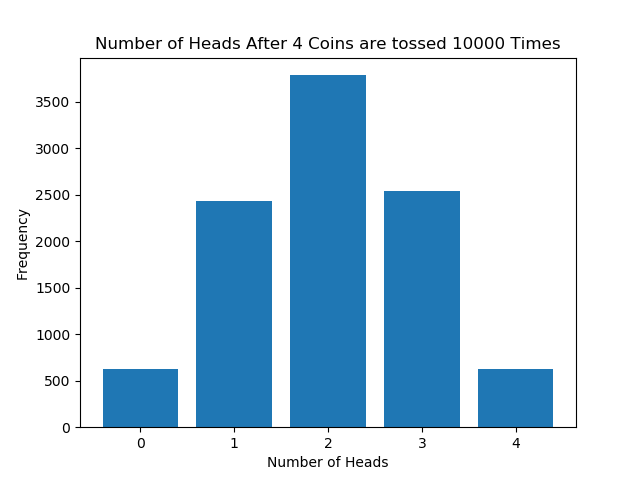
\includegraphics[scale=0.35]{coin_toss_results_10000.png}
            \caption{Results of tossing 4 coins 10 times.}
        \end{subfigure}
        \begin{subfigure}{0.35\textwidth}
            \centering
            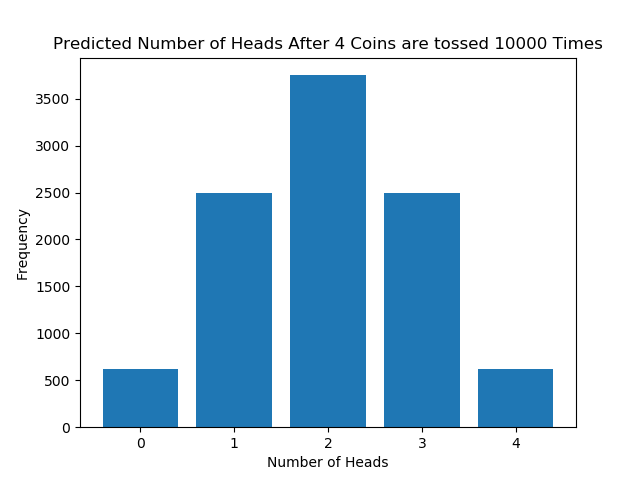
\includegraphics[scale=0.35]{coin_toss_prediction_10000.png}
            \caption{Predicted number of heads for tossing 4 coins 10 times.}
        \end{subfigure}
        \caption{Sample distribution vs. population distribution for counting the number of heads in four coin tosses.}
        \label{fig:10000 repeats}
    \end{figure}
    What we have here is that if \(f_n(X)\) is the number of times that \(X\) heads occurs in \(n\) coin tosses and \(N\) is the number of repeats then we expect
    \[\lim_{N\to\infty} \frac{f_n(X)}{N} = P_n(X).\]
    
    In the case of a continuous random variable, \(x\), then all of the above holds if we `bin' the results.
    By this we mean choose values, \(x_i\), of \(x\) and group the results into ranges around these values.
    This has been done in figure~\ref{fig:binned continuous sample}.
    \begin{figure}[ht]
        \centering
        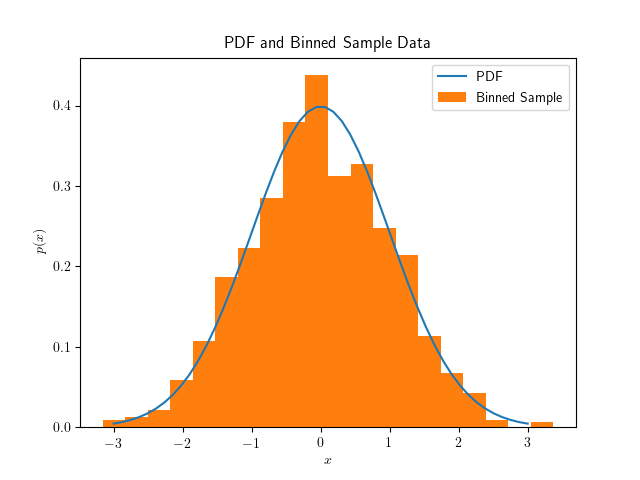
\includegraphics[scale=0.5]{binned_continuous_sample.png}
        \caption{A sample of a continuous random variable, binned, normalised, and plotted against the underlying \acrshort{pdf}.}
        \label{fig:binned continuous sample}
    \end{figure}
    Again we expect the normalised sample data to tend to the probability as we increase the number of repeats.
    If \(f(x_i)\) is the frequency with which data falls in the bin centred on \(x_i\), \(\Delta x\) is the width of the bin, and \(N\) is the size of the set of sample data then we expect
    \[\lim_{N\to\infty} \frac{f(x_i)}{N\Delta x} = p(x)\]
    
    \subsection{Multivariate Distributions}
    Often we have two random variables.
    If \(X\) and \(Y\) are discrete random variables then we can define a joint probability distribution, \(P\), by specifying \(P(X_i, Y_j)\) for all possible values of \(X_i\) and \(Y_j\).
    If instead \(x\) and \(y\) are continuous random variables then we define \(p(x, y)\) such that the probability that \((x, y)\in[x, x + \dd{x}]\times[y, y + \dd{y}]\) is \(p(x, y)\dd{x}\dd{y}\).
    
    Either way we end up with a three dimensional function (in the sense that we have two inputs and an output so need three dimensions to visualise it).
    We could use heat maps, contour maps, or 3D plots.
    \begin{figure}[ht]
        \centering
        \begin{subfigure}{0.35\textwidth}
            \centering
            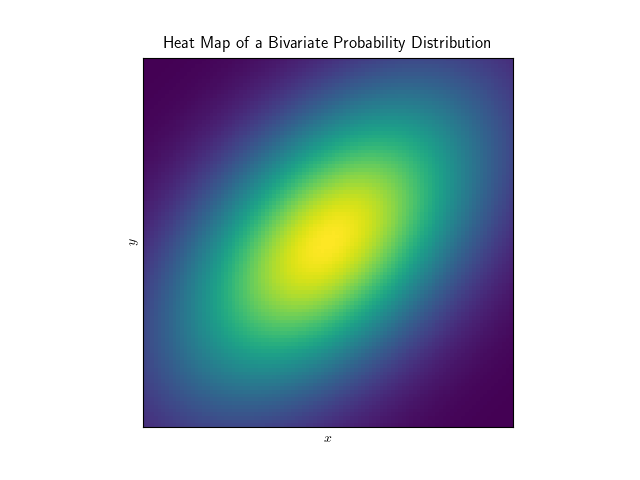
\includegraphics[scale=0.35]{bivariate_heat_map.png}
            \caption{A bivariate probability density function heat map.}
            \label{fig:bivariate heat map}
        \end{subfigure}
        \begin{subfigure}{0.35\textwidth}
            \centering
            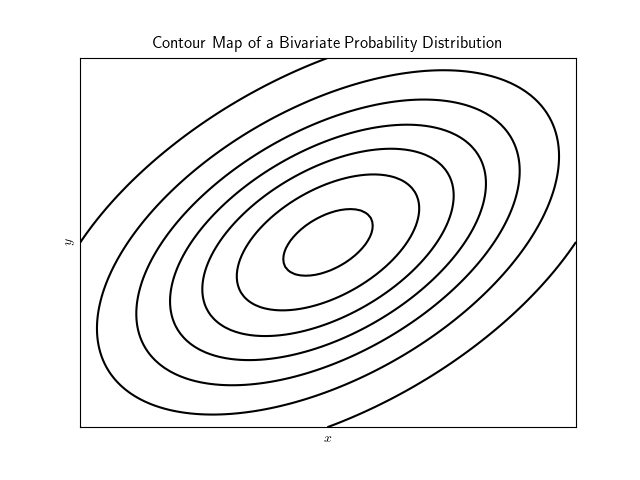
\includegraphics[scale=0.35]{bivariate_contour_map.png}
            \caption{A bivariate probability density function contour map.}
        \end{subfigure}
        \begin{subfigure}{0.35\textwidth}
            \centering
            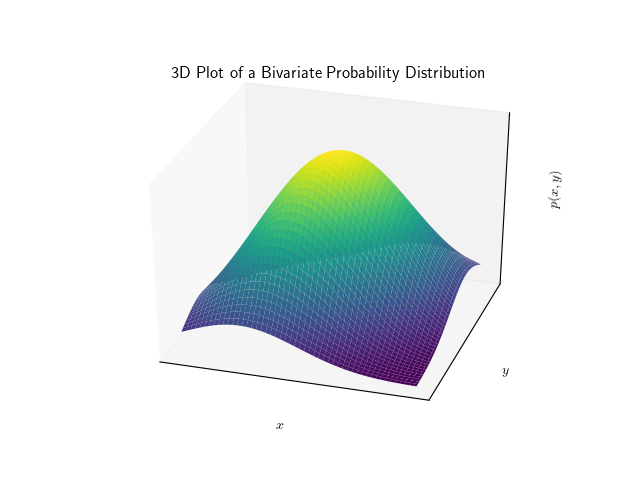
\includegraphics[scale=0.4]{bivariate_3d_plot.png}
            \caption{A bivariate probability density function plot.}
        \end{subfigure}
        \caption{Different ways to plot a bivariate probability distribution.}
    \end{figure}
    One question that we might logically ask is what information can we extract about one random variable from a joint probability distribution.
    The answer is that it depends what we want.
    If we want to know about one variable and have knowledge of the other then we get a different answer to if we want to know about one variable and don't care about the other.
    In the first case we get a conditional distribution and in the second a marginal distribution.
    
    \subsubsection{Conditional Distributions}
    If \((x, y)/(X, Y)\) is a pair of continuous/discrete random variables with probability density/probability given by \(p/P\) and we want information about \(x/X\) then one thing that we could do is fix \(y=y^*/Y=Y_j\) and look at \(p(x, y^*)/P(X, Y_j)\).
    This is like taking a slice through the data at this fixed value.
    We can define a new probability distribution/probability based off of this.
    In the continuous case we have
    \[q_{y^*}(x) = q(x|y^*) = \frac{p(x, y^*)}{\int p(x, y^*)\,\dd{x}}\]
    here the integral ensures that this is properly normalised.
    In the discrete case we have
    \[Q_j(X_i) = Q(X_i|Y_j) = \frac{P(X_i, Y_j)}{\sum_{j}P(X_i, Y_j)}.\]
    These are called conditional distributions because we are looking at distributions for \(x/X\) given a condition of some particular \(y/Y\) value.
    
    \begin{example}
        \begin{table}[ht]
            \centering
            \begin{tabular}{ccccccccc|c}
                &\multicolumn{8}{c}{Head Breadth/\si{\centi\metre}}&\\
                Head Length/\si{\centi\metre} & 13 & 13.5 & 14 & 14.5 & 15  & 15.5 & 16 & 16.5 & Total\\
                16    & 0 & 0 & 0 & 0 & 1 & 0 & 0 & 0 & 1\\
                16.5  & 0 & 0 & 1 & 0 & 1 & 0 & 0 & 0 & 2\\
                17    & 0 & 5 & 4 & 4 & 1 & 0 & 0 & 0 & 14\\
                17.5  & 1 & 8 & 17 & 15 & 11 & 2 & 0 & 0 & 54\\
                18    & 0 & 6 & 55 & 119 & 74 & 14 & 1 & 0 &269\\
                \rowcolor{lightgray}
                18.5  & 0 & 5 & 108 & 264 & 234 & 75 & 6 & 1 & 693\\
                19    & 0 & 10 & 72 & 360 & 400 & 156 & 26 & 2 & 1026\\
                19.5  & 0 & 1 & 28 & 174 & 239 & 160 & 36 & 7 & 645\\
                20    & 0 & 2 & 4 & 31 & 86 & 100 & 24 & 2 & 249\\
                20.5  & 0 & 0 & 1 & 4 & 17 & 17 & 5 & 0 & 44\\
                21    & 0 & 0 & 1 & 0 & 0 & 1 & 0 & 1 & 3\\\hline
                Total & 1 & 37 & 291 & 971 & 1064 & 525 & 98 & 13 & 3000
            \end{tabular}
            \caption{Head length vs. head breadth, all measurements in \si{\centi\metre}, headings refer to lower bound of range and all ranges go up to the next heading.}
            \label{tab:head measurements}
        \end{table}
        Table~\ref{tab:head measurements} has a list of measurements of head breadth and length.
        These were collected from 3000 prisoners in a study into phrenology--the idea that the shape of someone's head can be used to predict certain traits.
        Needless to say this is not true and the whole field was used to justify racism but data is data and we can still do some statistics on it.
        
        Say we know that someone's head is \SI{18.5}{\centi\metre} long.
        What is the probability distribution for their head breadth?
        Assuming that their head breadth falls within the values measured in this study we look specifically at the row for head length \SI{18.5}{\centi\metre}.
        The probability of any particular head breadth, given a head length of \SI{18.5}{\centi\metre} is the value in the relevant column divided by the total of the row, in this case 693.
        For example the probability of having a head breadth between \SIlist{14;14.5}{\centi\metre} given a head length of \SI{18.5}{\centi\metre} is
        \[P(14~\text{to}~14.5) = \frac{108}{693} = 0.156.\]
    \end{example}
    \subsubsection{Marginal Distribution}
    If we have no knowledge of \(y/Y\) then the best that we can do is a marginal distribution.
    All that we do here is start by choosing a particular value of \(y/Y\) and counting all the occurrences in cells consistent with that value.
    This corresponds to adding the values in that row/column.
    Going back to the example of table~\ref{tab:head measurements} the case where we choose \(x \in [14.5, 15)\) gives us a sum of 291.
    We repeat this for different \(x\) values to get the bottom row of table~\ref{tab:head measurements}.
    This process is known as marginalising over \(y\) as the results are written in the margin of the table.
    We end up with the distribution
    \[q(x) = \int p(x, y)\,\dd{y}\]
    for a continuous random variable and
    \[Q(X_j) = \sum_{i} P(X_i, Y_j)\]
    for a discrete random variable.
    
    \subsection{Dependence}
    Note how the ellipse in the bivariate distribution shown in figure~\ref{fig:bivariate heat map} is tilted.
    This means that if we take slices at different \(y\) values the most likely \(x\) value (represented by the lightest part of the heat map) changes.
    This means that there is some relation between the two variables \(x\) and \(y\).
    
    If there were no relation then we would expect the heat map to have two fold symmetry along the horizontal and vertical.
    If \(x\) and \(y\) are independent continuous random variables then it is possible to write the probability density function as \(p(x, y) = f(x)g(y)\) where \(f\) and \(g\) are the marginal distributions of \(x\) and \(y\) respectively.
    We could do the same for discrete variables also.
    
    \subsection{Characterising Distributions}
    \subsubsection{Mean}
    Suppose \(x\) is a continuous random variable with \acrshort{pdf} \(p\).
    What is the typical value of \(x\)?
    It depends what you mean by this:
    \begin{itemize}
        \item If you mean the value where \(p\) is maximised then this is known as the mode.
        The problem is that the mode depends on how we bin the data.
        \item If you mean the value that has half the values below it and half the values above it then this is the median.
        The problem with the median is that is hard to work with.
        \item If you mean the average then this is the (arithmetic) mean.
        This is the most useful answer to this question.
    \end{itemize}
    It is important to distinguish between the mean of the sample, \(\bar{x}\), and the population, \(\mu\).
    The sample mean is
    \[\bar{x} = \frac{\sum_i x_i}{N}\]
    where the sample is \(\{x_i\st i=1, \dotsc, N\}\).
    Note that this is still the sample even if \(x\) is continuous as the sample is simply a set of measurements.
    The population mean depends on whether we are dealing with a discrete or continuous random variable.
    In the case of a continuous random variable it is
    \[\mu = \frac{\int xp(x)\,\dd{x}}{\int p(x)\,\dd{x}}\]
    for a discrete random variable it is
    \[\mu = \frac{\sum_i X_i}{n}\]
    where \(\{X_i\st i = 1, \dotsc, n\}\) is the sample space.
    In general we expect that as \(N \to \infty\) \(\bar{x} \to \mu\).
    
    \subsubsection{Dispersion}
    Another thing that we might want to know is the spread of the values.
    The naive approach to characterising this would be to consider the, deviation, that is the difference between the mean and each value in the sample, \(x_i - \bar{x}\).
    The problem with this is that the logical way to account for all measurements, \(x_i\), is to take the average deviation of all points.
    However for a symmetric distribution \(x_i\) is just as likely to be either side of \(\bar{x}\) so we would expect the sum in the average to come out to approximately zero no matter the spread.
    
    To get rid of this issue we need to get rid of negatives.
    The most common way to do this is to take the square of the deviation and then average.
    This gives the variance.
    The sample variance is
    \[V = s^2 = \frac{\sum_i (x_i - \bar{x})}{N}.\]
    The population variance of a continuous variable is
    \[\Var(x) = \sigma^2 = \int (x - \mu)^2p(x)\,\dd{x},\]
    whereas for a discrete variable it is
    \[\sigma^2 = \frac{\sum_i (X_i - \mu)}{n}.\]
    Again as \(N\to\infty\) we expect \(s^2 \to \sigma^2\).
    
    It is common to use the square root of the variance, known as the standard deviation, dispersion, or \acrfull{rms} deviation.
    Sometimes the dimensionless ratio \(s/\bar{x}\) for a sample. or \(\sigma/\mu\) for a population, is used, it is called the coefficient of variation.
    It is useful for comparing different distributions due to being dimensionless.
    
    Yet another measurement that we may consider is what range of values of \(x\) it takes to encompass a certain proportion of the outcomes of experiment.
    For example we may want \SI{90}{\percent} of values to fall in this range.
    What we do is integrate \(p(x)\) and choose \(x_1\) and \(x_2\) such that
    \[P_\mathrm{int} = \int_{x_1}^{x_2}p(x)\,\dd{x}.\]
    Here \(P_\mathrm{int}\) is the proportion of values that we require to be in \([x_1, x_2]\).
    For example \(P_\mathrm{int} = 0.9\).
    We haven't yet solved the problem as \(x_1\) and \(x_2\) will not be unique.
    There are two common choices.
    One is to choose \([x_1, x_2]\) to be centred on the mean so we have \(x_1 = \mu - x_3\) and \(x_2 = \mu + x_3\).
    There is only one value of \(x_3\) such that the integral above holds.
    The other choice is to choose \(x_2 = \infty\) or some maximum possible value (or equivalently choose \(x_1 = -\infty\) or some minimum possible value) and then we are looking for what value of \(x_1\) \((x_2)\) we need to choose to have \(P_\mathrm{int}\) of the values greater than \(x_1\) (less than \(x_2\)).
    
    
    \subsubsection{Bivariate Distributions}
    If we have a bivariate distribution, \(p(x, y)\), we can find the mean of \(x\) and \(y\), denoted \(\mu_x\) and \(\mu_y\) respectively, as well as the standard deviations, denoted \(\sigma_x^2\) and \(\sigma_y^2\) respectively.
    To do this we marginalise over \(x\) and \(y\) to get their marginalised probability distributions and proceeding with the normal computations using these marginalised distributions.
    
    We can also characterise how much the variables \(x\) and \(y\) are related.
    The simplest quantity that does this is the covariance.
    It gives a measure of how much \(x\) will get bigger if \(y\) gets bigger.
    It is zero if \(x\) and \(y\) are independent.
    It is negative if \(x\) gets smaller when \(y\) gets bigger.
    It is defined for a sample distribution as
    \[s_{xy} = \frac{1}{N}\sum_{i} (x_i - \bar{x})(y_i - \bar{y})\]
    Then for the parent distribution we have
    \[\Cov(x, y) = \sigma_{xy} = \lim_{N\to\infty} s_{xy}.\]
    The matrix
    \[
        \sigma = 
        \begin{pmatrix}
            \sigma_{x_1}^2 & \sigma_{x_1x_2} & \dotsc\\
            \sigma_{x_2x_1} & \sigma_{x_2}^2 & \dotsc\\
            \vdots & \vdots & \ddots
        \end{pmatrix}
    \]
    is called the covariance matrix and encodes the dependence of random variables \(x_i\).
    
    \section{Expected Value}
    Given a random variable we can assign to it an average value, that is the mean value that we expect if we measure the variable repeatedly.
    For a discrete variable, \(X\), the expected value is
    \[E[X] = \expected{X} = \sum_i X_iP(X_i).\]
    For a continuous variable, \(x\), the expected value is
    \[E[x] = \expected{x} = \int xp(x)\dd{x}.\]
    A function, \(f\), of a random variable, \(x\), is itself a random variable and its expected value is
    \[E[f(x)] = \int f(x)p(x)\dd{x}.\]
    One important case is for random variables \(x\) and \(y\) and constants \(a\) and \(b\)
    \[E[ax + by] = aE[x] + bE[y].\]
    
    \subsection{Moments of a Distribution}
    For a random variable \(x\) with \acrshort{pdf} \(p\) the \(n\)th moment of \(x\) is defined as the expected value of \(x^n\):
    \begin{align*}
        m_n &= E[x^n] = \int x^n p(x)\dd{x}\\
        m_0 &= E[x^0] = \int p(x)\dd{x} = 1\\
        m_1 &= E[x^1] = \int xp(x)\dd{x} = \mu
    \end{align*}
    A more useful value from here on is the centred moments which are obtained by shifting the origin of \(x\) to the mean, \(\mu\):
    \begin{align*}
        \mu_n &= E[(x - \mu)^n] = \int(x - \mu)^np(x)\dd{x}\\
        \mu_0 &= E[(x - \mu)^1] = E[1] = 1\\
        \mu_1 &= E[(x - \mu)^1] =  E[x] - E[\mu] = \mu - \mu = 0\\
        \mu_2 &= E[(x - \mu)^2] = \int(x - \mu)^2p(x)\dd{x} = \sigma^2
    \end{align*}
    For comparison between distributions it makes sense to define a dimensionless constant, \(\alpha_n = \mu_n/\sigma^n\).
    For example the skewness of a distribution, a measure of asymmetry, is \(\alpha_3\) and a moderately skewed distribution would have \(\abs{\alpha_3}\) somewhere between 0.5 and 1.
    The extremely skewed exponential distribution has a skewness of \(\alpha_3 = 2\).
    The sign of \(\alpha_3\) tells us which way the distribution is skewed, if \(\alpha_3 > 0\) then the right hand side of the distribution tails away slowly and the left is steep.
    The opposite is true if \(\alpha_3 < 0\).
    
    Kurtosis is a measure of how peaky a distribution is.
    It is defined as \(\alpha_4\).
    It can take any value from 1 to \(\infty\).
    The Gaussian distribution has a kurtosis of \(\alpha_4 = 3\).
    It is common to define the excess kurtosis as \(\alpha_4 - 3\).
    If the excess kurtosis is positive then the distribution is peaky, known as leptokurtic.
    If the excess kurtosis is negative then the distribution is squat, known as platykurtic.
    
    We can also define the sample moments as
    \[\mu_n = \frac{1}{N}\sum_{i=1}^{N} (x_i - \bar{x})^n.\]
    
    One useful result is that
    \[\sigma^2 = E[(x - \mu)^2] = E[(x - E[x])^2] = E[x^2 - 2xE[x] + E[x]^2] = E[x^2] = 2E[x]E[x] + E[x]^2 = E[x^2] - E[x]^2.\]
    Another useful result is that
    \[E[(x - \mu_x)(y - \mu_y)] = \Cov(x, y) = \sigma_{xy}.\]
    
    \subsection{Transformation of Probability Distributions}
    If we have a random variable, \(x\), then a function of that variable, \(z = z(x)\), is also a random variable.
    If \(f\) is the \acrshort{pdf} of \(x\) then the \acrshort{pdf}, \(g\), of \(z\) is
    \[g(z) = f(x)\dv{x}{z}.\]
    We can do something similar for the multivariate case but it requires a Jacobian.
    
    The most common question we might ask is if we know \(\sigma_x^2\) then what is \(\sigma_z^2\)?
    
    \subsubsection{Transformation of Variance: Univariate Case}
    The variance of \(z\) is
    \[\sigma_z^2 = \lim_{N\to\infty}\frac{1}{N}\sum_{i=1}^{N} (z_i - \bar{z})^2.\]
    To first order we have
    \[z_i - \bar{z} = (x_i - \bar{x})\dv{z}{x}.\]
    This means
    \[\sigma_z^2 = \lim_{N\to\infty}\frac{1}{N}\sum_{i=1}^{N} (x_i - \bar{x})^2\left(\dv{z}{x}\right)^2.\]
    Identifying the first part as \(\sigma_x^2\) we see that
    \[\sigma_z = \sigma_x\dv{z}{x}.\]
    
    \subsubsection{Transformation of Variance: Bivariate Case}
    If \(z = z(x, y)\) then to first order
    \[z_i - \bar{z} = (x_i - \bar{x})\pdv{z}{x} + (y_i - \bar{y})\pdv{z}{y}.\]
    The variance in \(z\) is then
    \begin{align*}
        \sigma_z^2 &= \lim_{N\to\infty}\frac{1}{N}\sum_{i=1}^{N} \left[(x_i - \bar{x})\pdv{z}{x} + (y_i - \bar{y})\pdv{z}{y}\right]^2\\
        &= \lim_{N\to\infty}\frac{1}{N}\sum_{i=1}^{N} \left[(x_i - \bar{x})^2\left(\pdv{z}{x}\right)^2 + (y_i - \bar{y})^2\left(\pdv{z}{y}\right)^2 + 2(x_i - \bar{x})(y_i - \bar{y})\pdv{z}{x}\pdv{z}{y}\right]\\
        &= \sigma_x^2\left(\pdv{z}{x}\right)^2 + \sigma_y^2\left(\pdv{z}{y}\right)^2 + 2\sigma_{xy}\left(\pdv{z}{x}\right)\left(\pdv{z}{y}\right).
    \end{align*}
    In the case that \(x\) and \(y\) are independent this reduces to
    \[\sigma_z^2 = \sigma_x^2\left(\pdv{z}{x}\right)^2 + \sigma_y^2\left(\pdv{z}{y}\right)^2.\]
    In the specific case that \(z = x + y\) for independent \(x\) and \(y\) this reduces further to
    \[\sigma_z^2 = \sigma_x^2 + \sigma_y^2.\]
    We see that uncertainties add in quadrature.
    
    We can easily compute more examples:
    \[
        \begin{array}{ll}
            f(x, y) = ax \pm by & \sigma_f^2 = a^2\sigma_x^2 + b^2\sigma_y^2\\
            f(x, y) = xy~\text{or}~\frac{x}{y} & \left(\frac{\sigma_f}{f}\right)^2 = \left(\frac{\sigma_x}{x}\right)^2 + \left(\frac{\sigma_y}{y}\right)^2\\
            f(x) = ax^{\pm b} & \frac{\sigma_f}{f} = b\frac{\sigma_x}{x}\\
            f(x) = a^{\pm bx} & \frac{\sigma_f}{f} = b\ln(a\sigma_x)\\
            f(x) = ae^{\pm b} & \frac{\sigma_f}{f} = b\sigma_x\\
            f(x) = a\ln(\pm bx) & \sigma_f = a\frac{\sigma_x}{x}\\
        \end{array}
    \]